\documentclass[10pt]{article}

\usepackage[letterpaper, margin=1in]{geometry}
\usepackage{graphicx}
\usepackage{listings}
\usepackage{verbatim}

\title{An Abjad-Book Example}
\author{Josiah Wolf Oberholtzer}

\begin{document}

\maketitle

\begin{abstract}
This is an abstract.
\end{abstract}

\section{First section}

Blah blah blah.

\begin{comment}
<abjad>
from abjad import *
staff = Staff("c'4 d'4 e'4 f'4")
show(staff)
</abjad>
\end{comment}

%%% ABJADBOOK START %%%
\begin{lstlisting}
>>> from abjad import *
>>> staff = Staff("c'4 d'4 e'4 f'4")
>>> show(staff)
\end{lstlisting}
\noindent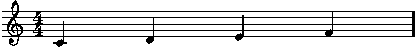
\includegraphics{assets/lilypond-3947a1689e36c26dfc1db5d199985257.pdf}
%%% ABJADBOOK END %%%

\section{Second section}

Blah blah blah.

\begin{comment}
<abjad>
graph(staff)
</abjad>
\end{comment}

%%% ABJADBOOK START %%%
\begin{lstlisting}
>>> graph(staff)
\end{lstlisting}
\noindent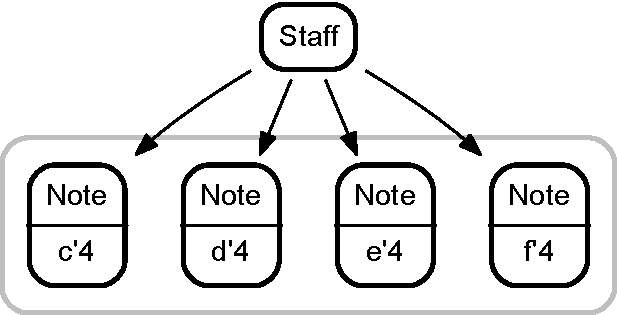
\includegraphics[scale=0.4,]{assets/graphviz-3b34c87165f86ad4d24e10086c571779.pdf}
%%% ABJADBOOK END %%%

\section{Third section}

Blah blah blah.

\begin{comment}
<abjad>
for note in staff:
    print(format(note))
</abjad>
\end{comment}

%%% ABJADBOOK START %%%
\begin{lstlisting}
>>> for note in staff:
...     print(format(note))
...
c'4
d'4
e'4
f'4
\end{lstlisting}
%%% ABJADBOOK END %%%

\end{document}